\documentclass[12pt,mathserif,compress]{beamer}

\beamertemplateshadingbackground{black!5}{black!20}
\usepackage[spanish]{babel}
\usepackage{times}
\usepackage[T1]{fontenc}
\usepackage[utf8]{inputenc}
\usepackage{graphicx}
\usepackage{tikz}
\usepackage{listings}

%\usepackage{pgfpages}
%\pgfpagesuselayout{4 on 1}[a4paper,border shrink=5mm]

\renewcommand\shorthandsspanish{}
\noextrasspanish

\title{Python}
\author{Guillem Borrell i Nogueras}

\begin{document}

\lstset{language=Python,
  backgroundcolor=\color{black!10},
  numbers=left,
  basicstyle=\small\ttfamily,
  keywordstyle=\color{blue},
  extendedchars=true,
  inputencoding=utf8,
  showspaces=false}

\begin{frame}
\begin{center}
 
\includegraphics[width=9cm]{files/python-logo-generic.pdf}\\
 % python-logo-generic.pdf: 389x115 pixel, 72dpi, 13.72x4.06 cm, bb=0 0 389 115
\vspace{1cm}
Guillem Borrell i Nogueras\\

Físicas UCM, 18 Nov 2009
\end{center}

\end{frame}

\begin{frame}
  \frametitle{Antes de empezar}
  \begin{itemize}
  \item Guillem Borrell i Nogueras.
    \begin{itemize}
    \item  \url{http://guillemborrell.es/}
    \end{itemize}
  \item Ingeniero Aeronáutico
    \begin{itemize}
    \item Nunca me han gustado especialmente los aviones
    \end{itemize}
  \item Laboratorio de Mecánica de Fluidos Computacional
    \begin{itemize}
    \item Turbulencia en pared
    \end{itemize}
  \item Consultor de Englobe Technologies
    \begin{itemize}
    \item Supercomputación
    \end{itemize}
  \end{itemize}
\end{frame}

\begin{frame}
\frametitle{El software libre y un servidor}
\begin{itemize}
\item Empecé programando en Basic con un MSX y un monitor monocromo
  \textcolor{orange}{naranja}. Me gustaba.
\pause
\item Mis padres me compraron un PC con windows 3.11. Aprendí
  MS-DOS.
\pause
\item Windows 95 me hizo odiar el ordenador. Lo usaba para jugar al
  Civilization II.
\pause
\item En 3º un colega teleco me pasó un Red Hat 8.  Usé Octave para
  mis prácticas de Numérico II.
\end{itemize}
\end{frame}

\begin{frame}
\frametitle{Entonces llegó un verano de insomnio}
\begin{center}
 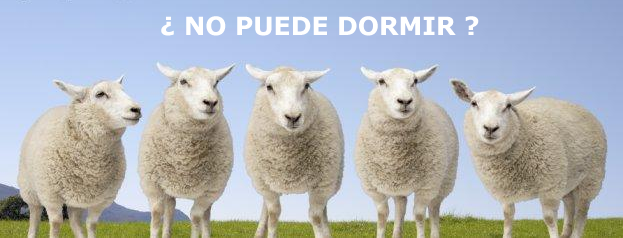
\includegraphics[width=\textwidth]{files/insomnio-ovejas.png}\\
\end{center}
\end{frame}

\begin{frame}
  \begin{center}
    Recordé lo bien que lo pasaba con el MSX de pequeño.
  \end{center}
\end{frame}

\begin{frame}
  \frametitle{Instalé un cluster casero en Gentoo Linux}
  \begin{center}
 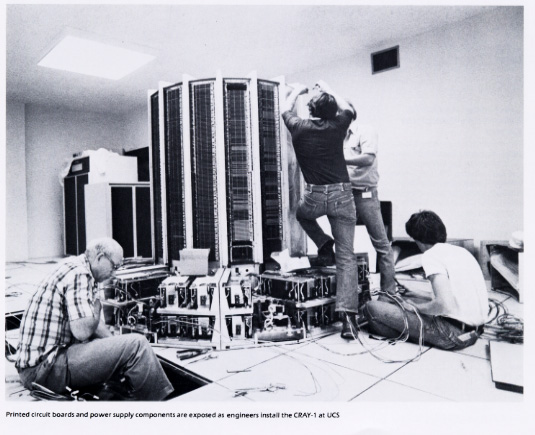
\includegraphics[width=0.8\textwidth]{files/ucs_Cray1_install.jpg}    
  \end{center}
\end{frame}

\begin{frame}
  \frametitle{Escribí un libro sobre Matlab y Octave}
  \begin{center}
  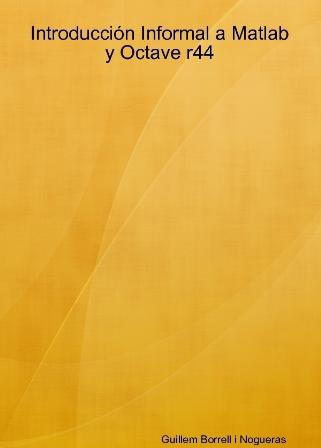
\includegraphics[height=0.6\textheight]{files/portada.jpg}    
  \end{center}
\end{frame}

\begin{frame}
  \begin{center}
    El insomnio no se fue, así que me tomé un año sabático.
  \end{center}
\end{frame}

\begin{frame}
  \frametitle{Aprendí cosas que no se enseñan en la Universidad}
Y menos aún en la Escuela de Aeronáuticos
\begin{itemize}
\item C y C++
\pause
\item Administración Linux
\pause
\item Redes
\pause
\item \textcolor{red}{\textbf{Python}}
\end{itemize}
\end{frame}

\begin{frame}
\frametitle{Python...}
\begin{center}
El lenguaje más versátil y consistente del mundo  
\end{center}

\end{frame}

\begin{frame}
  \frametitle{¿Qué es?}
Lenguaje de programación
\begin{itemize}
\item Interpretado
\item Dinámico
\item Tipado
\item Modular
\item Orientado a objetos
\item Ampliable
\item Consistente
\end{itemize}
\end{frame}

\begin{frame}
  \begin{center}
  ¿Qué significa consistencia?    
  \end{center}
\end{frame}

\begin{frame}
  \frametitle{The Zen of Python \#13}
  \begin{center}
      \textit{Debe haber una ---mejor si es sólo una--- manera obvia de
    hacer algo}
  \end{center}
\end{frame}

\end{document}

